\documentclass{article}

\usepackage[a4paper, total={7in, 9in}]{geometry}
\pagestyle{empty} % Prevent relative page numbers

%%%%%%%%%%%%%%%%%%%%%%%%%%%%%%%%%%%%%%
%% Default definitions 
%% Define listings format
\usepackage{xcolor} % Required for listings color definitions
\definecolor{Brown}{cmyk}{0,0.81,1,0.60}
\definecolor{OliveGreen}{cmyk}{0.64,0,0.95,0.40}
\definecolor{CadetBlue}{cmyk}{0.62,0.57,0.23,0}
\definecolor{lightlightgray}{gray}{0.9}

\usepackage{listings} % computer code language formatting

\lstdefinestyle{tex-style} {
	language=[LaTeX]TeX,                    % Code langugage
	basicstyle=\ttfamily,                   % Code font, Examples: \footnotesize, \ttfamily
	%keywordstyle=\color{OliveGreen},        % Keywords font ('*' = uppercase)
	commentstyle=\color{gray},              % Comments font
	numbers=none,                           % Line nums position
	numberstyle=\tiny,                      % Line-numbers fonts
	stepnumber=1,                           % Step between two line-numbers
	numbersep=5pt,                          % How far are line-numbers from code
	backgroundcolor=\color{lightlightgray}, % Choose background color
	frame=single,                             % A frame around the code
	tabsize=2,                              % Default tab size
	captionpos=b,                           % Caption-position = bottom
	breaklines=true,                        % Automatic line breaking?
	breakatwhitespace=false,                % Automatic breaks only at whitespace?
	showspaces=false,                       % Dont make spaces visible
	showtabs=false,                         % Dont make tabls visible
	columns=flexible,                       % Column format
	morekeywords={__global__, __device__}  % CUDA specific keywords
}
\lstnewenvironment{latex}
{\lstset{language=[LaTeX]TeX}}
{}
\lstset{style=tex-style}

%% Define URL format
\usepackage[hyphens]{url}
\usepackage{hyperref}
\hypersetup{
	colorlinks=true,
	citecolor=black,
	filecolor=black,
	linkcolor=blue,
	urlcolor=blue
}

\setlength\parindent{0pt}


%%%%%%%%%%%%%%%%%%%%%%%%%%%%%%%%%%%%%%
%% Example-specific packages
\usepackage{pgfplots}

%%%%%%%%%%%%%%%%%%%%%%%%%%%%%%%%%%%%%%
%% Example-specific preamble
\makeatletter
\def\pgfmathstoreseed#1{\let#1\pgfmath@rnd@z}
\let\pgfmathrestoreseed\pgfmathsetseed
\makeatother


\begin{document}

\section*{Adding Noise to Plots}

\subsection*{Description}
Sometimes realistic noise needs to be added to function plots. The following code demonstrates that.

The \verb|\pgfmathstoreseed{arg1}| and \verb|\pgfmathrestoreseed| can be used to manipulate the random number generator seed.

The \verb|rand| function returns uniform noise. It would be nice to find some native command for Gaussian, white, etc noises.

\subsection*{Sources}
\url{https://tex.stackexchange.com/questions/144272/noisy-analogue-waveform-in-tikz}\\
\url{https://tex.stackexchange.com/questions/126838/plotting-a-random-function-fx-and-fxsinx-with-tikz}

\subsection*{Used Packages}
\verb|pgfplots|

\subsection*{Preamble}
\begin{latex}
%%%%%%%%%%%%%%%%%%%%%%%%%%%%%%%%%%%%%%
%% Example-specific packages
\usepackage{pgfplots}

%%%%%%%%%%%%%%%%%%%%%%%%%%%%%%%%%%%%%%
%% Example-specific preamble
\makeatletter
\def\pgfmathstoreseed#1{\let#1\pgfmath@rnd@z}
\let\pgfmathrestoreseed\pgfmathsetseed
\makeatother
\end{latex}

\subsection*{Document}
\begin{latex}
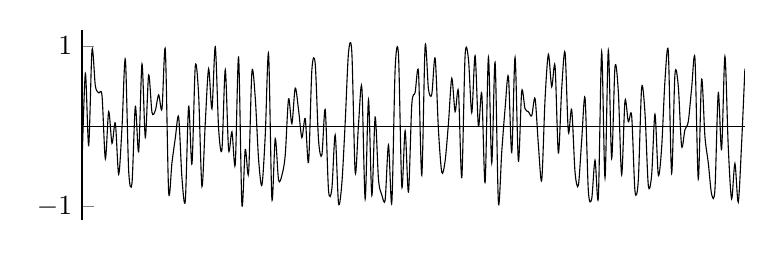
\begin{tikzpicture}[samples=200, domain=0:5*360]
\begin{axis}[
width=10cm, height=4cm,
enlarge x limits=false,
xtick=\empty,
axis lines*=middle,
]
\pgfmathsetseed{126838}
\addplot [no markers, smooth] {rand};
\end{axis}
\end{tikzpicture}

\noindent
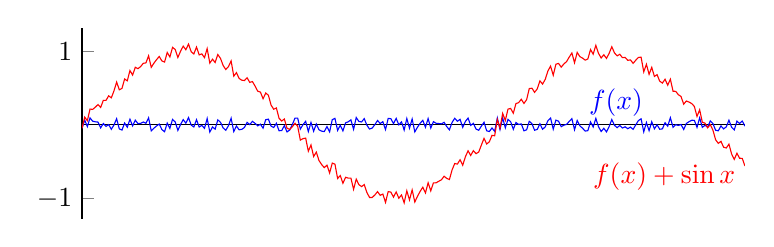
\begin{tikzpicture}[samples=250, domain=0:10]
\begin{axis}[
width=10cm, height=4cm,
enlarge x limits=false,
xtick=\empty,
axis lines*=middle,
]
\pgfmathsetseed{126838}
\addplot[color=blue] {rand/10};
\node[right] at (axis cs:7.5,0.3) {\color{blue}$f(x)$};
\pgfmathsetseed{126838}
\addplot[color=red] {rand/10 + sin (deg(x))};
\node[left] at (axis cs:10,-0.7) {\color{red}$f(x) + \sin x$};
\end{axis}
\end{tikzpicture}
\end{latex}

\subsection*{Result}

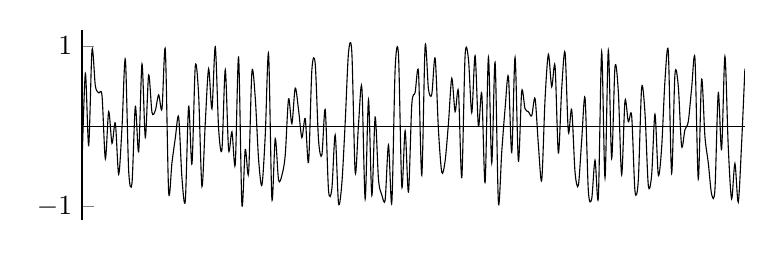
\begin{tikzpicture}[samples=200, domain=0:5*360]
	\begin{axis}[
	width=10cm, height=4cm,
	enlarge x limits=false,
	xtick=\empty,
	axis lines*=middle,
	]
	\pgfmathsetseed{126838}
	\addplot [no markers, smooth] {rand};
	\end{axis}
\end{tikzpicture}
 
\noindent
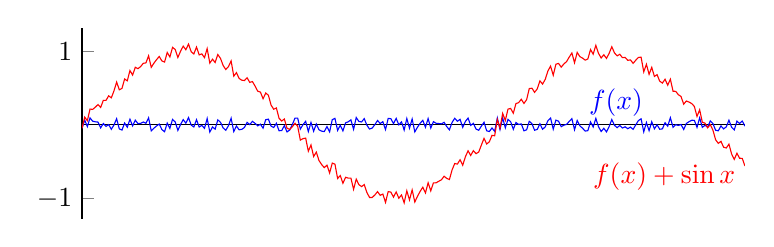
\begin{tikzpicture}[samples=250, domain=0:10]
\begin{axis}[
width=10cm, height=4cm,
enlarge x limits=false,
xtick=\empty,
axis lines*=middle,
]
\pgfmathsetseed{126838}
\addplot[color=blue] {rand/10};
\node[right] at (axis cs:7.5,0.3) {\color{blue}$f(x)$};
\pgfmathsetseed{126838}
\addplot[color=red] {rand/10 + sin (deg(x))};
\node[left] at (axis cs:10,-0.7) {\color{red}$f(x) + \sin x$};
\end{axis}
\end{tikzpicture}

\end{document}